\chapter{An Introduction to Groups}
\label{chapter:intro_groups}
\thispagestyle{empty}

%%----------------------------%%

One of the major topics of this course is \textbf{groups}.  The area of mathematics that is concerned with groups is called \textbf{group theory}. Loosely speaking, group theory is the study of symmetry, and in my opinion is one of the most beautiful areas in all of mathematics. It arises in puzzles, visual arts, music, nature, the physical and life sciences, computer science, cryptography, and of course, throughout mathematics.

%%----------------------------%%

\begin{section}{A First Example}\label{sec:first_example}

%%----------------------------%%

Let's begin our study by developing some intuition about what groups actually are.  To get started, we will explore the game Spinpossible\texttrademark, which used to be available for iOS and Android devices\footnote{If you'd like to play the game, try going here: \url{https://www.kongregate.com/games/spinpossible}.}.  The game is played on a $3\times 3$ board of scrambled tiles numbered 1 to 9, each of which may be right-side-up or up-side-down. The objective of the game is to return the board to the standard configuration where tiles are arranged in numerical order and right-side-up. This is accomplished by a sequence of ``spins", where a spin consists of rotating an $m\times n$ subrectangle by 180$^\circ$. The goal is to minimize the number of spins used.  The following figure depicts a scrambled board on the left and the solved board on the right.  The sequence of arrows is used to denote some sequence of spins that transforms the scrambled board into the solved board.

\begin{center}
\begin{tabular}{c}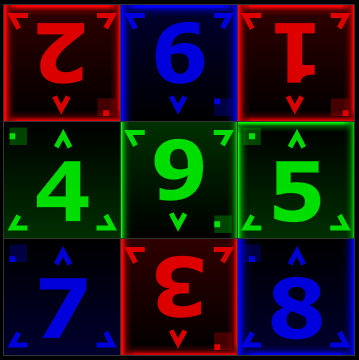
\includegraphics[width=1.5in]{scramble1.PNG}\end{tabular}
{\large $\xrightarrow{?} \cdots \xrightarrow{?}$}
\begin{tabular}{c}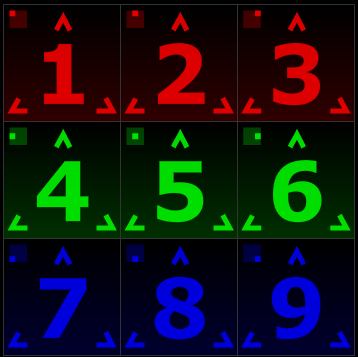
\includegraphics[width=1.5in]{scramble4.PNG}\end{tabular}
\end{center}

Let's play with an example.  Suppose we start with the following scrambled board.

\begin{center}
\begin{tikzpicture}[every node/.style={minimum size=.65cm}]
  \node [draw] (1) {\rotatebox{180}{$\underline{2}$}};
  \node [draw, right=0cm of 1] (2) {\rotatebox{180}{$\underline{9}$}};
  \node [draw, right=0cm of 2] (3) {\rotatebox{180}{$\underline{1}$}};
  \node [draw, below=0cm of 1] (4) {$\underline{4}$};
  \node [draw, right=0cm of 4] (5) {\rotatebox{180}{$\underline{6}$}};
  \node [draw, right=0cm of 5] (6) {$\underline{5}$};
  \node [draw, below=0cm of 4] (7) {$\underline{7}$};
  \node [draw, right=0cm of 7] (8) {\rotatebox{180}{$\underline{3}$}};
  \node [draw, right=0cm of 8] (9) {$\underline{8}$};
\end{tikzpicture}
\end{center}

\noindent The underlines on the numbers are meant to help us tell whether a tile is right-side-up or up-side-down.  Our goal is to use a sequence of spins to unscramble the board.  Before we get started, let's agree on some conventions.  When we refer to \emph{tile $n$}, we mean the actual tile that is labeled by the number $n$ regardless of its position and orientation on the board.  On the other hand, \emph{position $n$} will refer to the position on the board that tile $n$ is supposed to be in when the board has been unscrambled.  For example, in the board above, tile 1 is in position 3 and tile 7 happens to be in position 7.  

It turns out that there are multiple ways to unscramble this board, but I have one particular sequence in mind.  First, let's spin the rectangle determined by the two rightmost columns.  Here's what we get.  I've shaded the subrectangle that we are spinning.

\begin{center}
\begin{tabular}{c}
\begin{tikzpicture}[every node/.style={minimum size=.65cm}]
  \node [draw] (1) {\rotatebox{180}{$\underline{2}$}};
  \node [draw, fill=blue!40, right=0cm of 1] (2) {\rotatebox{180}{$\underline{9}$}};
  \node [draw, fill=blue!40, right=0cm of 2] (3) {\rotatebox{180}{$\underline{1}$}};
  \node [draw, below=0cm of 1] (4) {$\underline{4}$};
  \node [draw, fill=blue!40, right=0cm of 4] (5) {\rotatebox{180}{$\underline{6}$}};
  \node [draw, fill=blue!40, right=0cm of 5] (6) {$\underline{5}$};
  \node [draw, below=0cm of 4] (7) {$\underline{7}$};
  \node [draw, fill=blue!40, right=0cm of 7] (8) {\rotatebox{180}{$\underline{3}$}};
  \node [draw, fill=blue!40, right=0cm of 8] (9) {$\underline{8}$};
\end{tikzpicture}
\end{tabular}
%
{\large $\rightarrow$}
%
\begin{tabular}{c}
\begin{tikzpicture}[every node/.style={minimum size=.65cm}]
  \node [draw] (1) {\rotatebox{180}{$\underline{2}$}};
  \node [draw, right=0cm of 1] (2) {\rotatebox{180}{$\underline{8}$}};
  \node [draw, right=0cm of 2] (3) {$\underline{3}$};
  \node [draw, below=0cm of 1] (4) {$\underline{4}$};
  \node [draw, right=0cm of 4] (5) {\rotatebox{180}{$\underline{5}$}};
  \node [draw, right=0cm of 5] (6) {$\underline{6}$};
  \node [draw, below=0cm of 4] (7) {$\underline{7}$};
  \node [draw, right=0cm of 7] (8) {$\underline{1}$};
  \node [draw, right=0cm of 8] (9) {$\underline{9}$};
\end{tikzpicture}
\end{tabular}
\end{center}

\noindent Okay, now let's spin the middle column.

\begin{center}
\begin{tabular}{c}
\begin{tikzpicture}[every node/.style={minimum size=.65cm}]
  \node [draw] (1) {\rotatebox{180}{$\underline{2}$}};
  \node [draw, fill=blue!40, right=0cm of 1] (2) {\rotatebox{180}{$\underline{8}$}};
  \node [draw, right=0cm of 2] (3) {$\underline{3}$};
  \node [draw, below=0cm of 1] (4) {$\underline{4}$};
  \node [draw, fill=blue!40, right=0cm of 4] (5) {\rotatebox{180}{$\underline{5}$}};
  \node [draw, right=0cm of 5] (6) {$\underline{6}$};
  \node [draw, below=0cm of 4] (7) {$\underline{7}$};
  \node [draw, fill=blue!40, right=0cm of 7] (8) {$\underline{1}$};
  \node [draw, right=0cm of 8] (9) {$\underline{9}$};
\end{tikzpicture}
\end{tabular}
%
{\large $\rightarrow$}
%
\begin{tabular}{c}
\begin{tikzpicture}[every node/.style={minimum size=.65cm}]
  \node [draw] (1) {\rotatebox{180}{$\underline{2}$}};
  \node [draw, right=0cm of 1] (2) {\rotatebox{180}{$\underline{1}$}};
  \node [draw, right=0cm of 2] (3) {$\underline{3}$};
  \node [draw, below=0cm of 1] (4) {$\underline{4}$};
  \node [draw, right=0cm of 4] (5) {$\underline{5}$};
  \node [draw, right=0cm of 5] (6) {$\underline{6}$};
  \node [draw, below=0cm of 4] (7) {$\underline{7}$};
  \node [draw, right=0cm of 7] (8) {$\underline{8}$};
  \node [draw, right=0cm of 8] (9) {$\underline{9}$};
\end{tikzpicture}
\end{tabular}
\end{center}

\noindent Hopefully, you can see that we are really close to unscrambling the board.  All we need to do is spin the rectangle determined by the tiles in positions 1 and 2.

\begin{center}
\begin{tabular}{c}
\begin{tikzpicture}[every node/.style={minimum size=.65cm}]
  \node [draw, fill=blue!40] (1) {\rotatebox{180}{$\underline{2}$}};
  \node [draw, fill=blue!40, right=0cm of 1] (2) {\rotatebox{180}{$\underline{1}$}};
  \node [draw, right=0cm of 2] (3) {$\underline{3}$};
  \node [draw, below=0cm of 1] (4) {$\underline{4}$};
  \node [draw, right=0cm of 4] (5) {$\underline{5}$};
  \node [draw, right=0cm of 5] (6) {$\underline{6}$};
  \node [draw, below=0cm of 4] (7) {$\underline{7}$};
  \node [draw, right=0cm of 7] (8) {$\underline{8}$};
  \node [draw, right=0cm of 8] (9) {$\underline{9}$};
\end{tikzpicture}
\end{tabular}
%
{\large $\rightarrow$}
%
\begin{tabular}{c}
\begin{tikzpicture}[every node/.style={minimum size=.65cm}]
  \node [draw] (1) {$\underline{1}$};
  \node [draw, right=0cm of 1] (2) {$\underline{2}$};
  \node [draw, right=0cm of 2] (3) {$\underline{3}$};
  \node [draw, below=0cm of 1] (4) {$\underline{4}$};
  \node [draw, right=0cm of 4] (5) {$\underline{5}$};
  \node [draw, right=0cm of 5] (6) {$\underline{6}$};
  \node [draw, below=0cm of 4] (7) {$\underline{7}$};
  \node [draw, right=0cm of 7] (8) {$\underline{8}$};
  \node [draw, right=0cm of 8] (9) {$\underline{9}$};
\end{tikzpicture}
\end{tabular}
\end{center}

\noindent Putting all of our moves together, here is what we have.

\begin{center}
\begin{tabular}{c}
\begin{tikzpicture}[every node/.style={minimum size=.65cm}]
  \node [draw] (1) {\rotatebox{180}{$\underline{2}$}};
  \node [draw, fill=blue!40, right=0cm of 1] (2) {\rotatebox{180}{$\underline{9}$}};
  \node [draw, fill=blue!40, right=0cm of 2] (3) {\rotatebox{180}{$\underline{1}$}};
  \node [draw, below=0cm of 1] (4) {$\underline{4}$};
  \node [draw, fill=blue!40, right=0cm of 4] (5) {\rotatebox{180}{$\underline{6}$}};
  \node [draw, fill=blue!40, right=0cm of 5] (6) {$\underline{5}$};
  \node [draw, below=0cm of 4] (7) {$\underline{7}$};
  \node [draw, fill=blue!40, right=0cm of 7] (8) {\rotatebox{180}{$\underline{3}$}};
  \node [draw, fill=blue!40, right=0cm of 8] (9) {$\underline{8}$};
\end{tikzpicture}
\end{tabular}
%
{\large $\rightarrow$}
%
\begin{tabular}{c}
\begin{tikzpicture}[every node/.style={minimum size=.65cm}]
  \node [draw] (1) {\rotatebox{180}{$\underline{2}$}};
  \node [draw, fill=blue!40, right=0cm of 1] (2) {\rotatebox{180}{$\underline{8}$}};
  \node [draw, right=0cm of 2] (3) {$\underline{3}$};
  \node [draw, below=0cm of 1] (4) {$\underline{4}$};
  \node [draw, fill=blue!40, right=0cm of 4] (5) {\rotatebox{180}{$\underline{5}$}};
  \node [draw, right=0cm of 5] (6) {$\underline{6}$};
  \node [draw, below=0cm of 4] (7) {$\underline{7}$};
  \node [draw, fill=blue!40, right=0cm of 7] (8) {$\underline{1}$};
  \node [draw, right=0cm of 8] (9) {$\underline{9}$};
\end{tikzpicture}
\end{tabular}
%
{\large $\rightarrow$}
%
\begin{tabular}{c}
\begin{tikzpicture}[every node/.style={minimum size=.65cm}]
  \node [draw, fill=blue!40] (1) {\rotatebox{180}{$\underline{2}$}};
  \node [draw, fill=blue!40, right=0cm of 1] (2) {\rotatebox{180}{$\underline{1}$}};
  \node [draw, right=0cm of 2] (3) {$\underline{3}$};
  \node [draw, below=0cm of 1] (4) {$\underline{4}$};
  \node [draw, right=0cm of 4] (5) {$\underline{5}$};
  \node [draw, right=0cm of 5] (6) {$\underline{6}$};
  \node [draw, below=0cm of 4] (7) {$\underline{7}$};
  \node [draw, right=0cm of 7] (8) {$\underline{8}$};
  \node [draw, right=0cm of 8] (9) {$\underline{9}$};
\end{tikzpicture}
\end{tabular}
%
{\large $\rightarrow$}
%
\begin{tabular}{c}
\begin{tikzpicture}[every node/.style={minimum size=.65cm}]
  \node [draw] (1) {$\underline{1}$};
  \node [draw, right=0cm of 1] (2) {$\underline{2}$};
  \node [draw, right=0cm of 2] (3) {$\underline{3}$};
  \node [draw, below=0cm of 1] (4) {$\underline{4}$};
  \node [draw, right=0cm of 4] (5) {$\underline{5}$};
  \node [draw, right=0cm of 5] (6) {$\underline{6}$};
  \node [draw, below=0cm of 4] (7) {$\underline{7}$};
  \node [draw, right=0cm of 7] (8) {$\underline{8}$};
  \node [draw, right=0cm of 8] (9) {$\underline{9}$};
\end{tikzpicture}
\end{tabular}
\end{center}
In this case, we were able to solve the scrambled board in 3 moves.  It's not immediately obvious, but it turns out that there is no way to unscramble the board in fewer than 3 spins.  However, there is at least one other solution that involves exactly 3 spins.

\begin{problem}\label{prob:number_spinpossible_boards}
How many scrambled $3\times 3$ Spinpossible boards are there?  To answer this question, you will need to rely on some counting principles such as factorials. In this context, we want to include the solved board as one of the scrambled boards---it's just not very scrambled.
\end{problem}

\begin{problem}\label{prob:counting_spins}
How many spins are there?
\end{problem}

It's useful to have some notation. Let $s_{ij}$ (with $i\leq j$) denote the spin that rotates the subrectangle that has tile $i$ in the upper-left corner and tile $j$ in the lower-right corner.  As an example, the sequence of spins that we used above to unscramble our initial scrambled board is
\[
s_{29}\to s_{28} \to s_{12}.
\]
It may not have occurred to you, but we can also rotate a single tile. Every spin of the form $s_{ii}$ is called a \emph{toggle}. For example, $s_{44}$ toggles the tile in position 4.

We can think of each spin as a function and since we are doing spins on top of spins, every sequence of spins corresponds to a composition of functions. We will follow the standard convention of function composition that says the function on the right goes first.  In this case, our previous sequence of spins becomes $s_{12} \circ s_{28}  \circ s_{29}$, which we abbreviate as $s_{12} s_{28} s_{29}$. This might take some getting used to, but just remember that it is just like function notation---stuff on the right goes first. We will refer to expressions like $s_{12} s_{28} s_{29}$ as \textbf{words} in the alphabet $\{s_{ij}\mid i\leq j\}$.  Our words will always consist of a finite number of spins.

Every word consisting of spins corresponds to a function that takes as input some scrambled board and returns a scrambled board. We say that the words ``act on" the scrambled boards. For each word, there is an associated net action. For example, the word $s_{12} s_{23} s_{12}$ corresponds to swapping the positions but not orientation of the tiles in positions 1 and 3.  You should take the time to verify this for yourself. Sometimes it is difficult to describe what the net action associated to a word is, but there is always some corresponding net action nonetheless.

It is worth pointing out that $s_{12} s_{23} s_{12}$ is not itself a spin.  However, sometimes a composition of spins will yield a spin.  For example, the net action of $s_{12} s_{11} s_{12}$ is toggling the tile in position 2.  That is, $s_{12} s_{11} s_{12}$ and $s_{22}$ are two different words that correspond to the same net action. In this case, we write $s_{12} s_{11} s_{12}=s_{22}$, where the equality is referring to the net action as opposed to the words themselves. The previous example illustrates that multiple words may represent the same net action. 

\begin{problem}\label{prob:3_different_spins}
Find a sequence of 3 spins that is different from the one we described earlier that unscrambles the following board. Write your answer as a word consisting of spins.
\begin{center}
\begin{tikzpicture}[every node/.style={minimum size=.65cm}]
  \node [draw] (1) {\rotatebox{180}{$\underline{2}$}};
  \node [draw, right=0cm of 1] (2) {\rotatebox{180}{$\underline{9}$}};
  \node [draw, right=0cm of 2] (3) {\rotatebox{180}{$\underline{1}$}};
  \node [draw, below=0cm of 1] (4) {$\underline{4}$};
  \node [draw, right=0cm of 4] (5) {\rotatebox{180}{$\underline{6}$}};
  \node [draw, right=0cm of 5] (6) {$\underline{5}$};
  \node [draw, below=0cm of 4] (7) {$\underline{7}$};
  \node [draw, right=0cm of 7] (8) {\rotatebox{180}{$\underline{3}$}};
  \node [draw, right=0cm of 8] (9) {$\underline{8}$};
\end{tikzpicture}
\end{center}
\end{problem}

\begin{problem}
What is the net action that corresponds to the word $s_{23} s_{12} s_{23}$? What can you conclude about $s_{23} s_{12} s_{23}$ compared to 
$s_{12} s_{23} s_{12}$?
\end{problem}

We can also use exponents to abbreviate.  For example, $s_2^2$ is the same as $s_2 s_2$ (which in this case has the net action of doing nothing) and $(s_1 s_2)^2$ is the same as $s_1 s_2 s_1 s_2$.

\begin{problem}\label{prob:braid_relation}
It turns out that there is an even simpler word (i.e., a shorter word) that yields the same net action as $(s_1 s_2)^2$. Can you find one?
\end{problem}

Define $\Spin_{3\times 3}$ to be the collection of net actions that we can obtain from words consisting of spins.  We say that the set of spins \textbf{generates} $\Spin_{3\times 3}$ and we refer to the set of spins as a \textbf{generating set} for $\Spin_{3\times 3}$.  

\begin{problem}
Suppose $s_{x_1}s_{x_2}\cdots s_{x_n}$ and $s_{y_1}s_{y_2}\cdots s_{y_m}$ are both words consisting of spins. Then the corresponding net actions, say $u$ and $v$, respectively, are elements of $\Spin_{3\times 3}$. Prove that the composition of the actions $u$ and $v$ is an element of $\Spin_{3\times 3}$.
\end{problem}

The previous problem tells us that the composition of two net actions from $\Spin_{3\times 3}$ results in another net action in $\Spin_{3\times 3}$. Formally, we say that $\Spin_{3\times 3}$ is \textbf{closed} under composition.

It is clear that we can construct an infinite number of words consisting of spins, but since there are a finite number of ways to rearrange the positions and orientations of the tiles of the $3\times 3$ board, there are only a finite number of net actions arising from these words.  That is, $\Spin_{3\times 3}$ is a finite set of functions.

\begin{problem}
Verify that $\Spin_{3\times 3}$ contains an \textbf{identity} function, i.e., a function whose net action is ``do nothing." What happens if we compose a net action from $\Spin_{3\times 3}$ with the identity?
\end{problem}

A natural question to ask is whether every possible scrambled Spinpossible board can be unscrambled using only spins.  In other words, is $\Spin_{3\times 3}$ sufficient to unscramble every scrambled board? It turns out that the answer is yes.

\begin{problem}\label{prob:kindergarten_algorthim}
Verify that $\Spin_{3\times 3}$ is sufficient to unscramble every scrambled board by describing an algorithm that will always unscramble a scrambled board.  It does not matter whether your algorithm is efficient.  That is, we don't care how many steps it takes to unscramble the board as long as it works in a finite number of steps.  Using your algorithm, what is the maximum number of spins required to unscramble any scrambled board?
\end{problem}

In a 2011 paper, Alex Sutherland and Andrew Sutherland (a father and son team) present a number of interesting results about Spinpossible and list a few open problems. You can find the paper at \url{http://arxiv.org/abs/1110.6645}. As a side note, Alex is one of the developers of the game and his father, Andrew, is a mathematics professor at MIT. Using a brute-force computer algorithm, the Sutherlands verified that every scrambled $3\times 3$ Spinpossible board can be solved in at most 9 moves. However, a human readable mathematical proof of this fact remains elusive.  By the way, mathematics is chock full of open problems and you can often get to the frontier of what is currently known without too much trouble.  Mathematicians are in the business of solving open problems.

Instead of unscrambling boards, we can act on the solved board with an action from $\Spin_{3\times 3}$ to obtain a scrambled board.  Problem~\ref{prob:kindergarten_algorthim} tells us that we can use $\Spin_{3\times 3}$ to get from the solved board to any scrambled board. In fact, starting with the solved board makes it clear that there is a one-to-one correspondence between net actions and scrambled boards.

\begin{problem}
What is the size of $\Spin_{3\times 3}$? That is, how many net actions are in $\Spin_{3\times 3}$?
\end{problem}

Let's make a couple more observations.  First, every spin is reversible. That is, every spin has an \textbf{inverse}.  In the case of Spinpossible, we can just apply the same spin again to undo it.  For example, $s_{12}^2$ is the same as doing nothing. This means that the inverse of $s_{12}$, denoted $s_{12}^{-1}$, is $s_{12}$ itself. Symbolically, we write $s_{12}^{-1}=s_{12}$. Remember that we are exploring the game Spinpossible---it won't always be the case that repeating an action will reverse the action. 

In the same vein, every sequence of spins is reversible. For example, if we apply $s_{12} s_{23}$ (i.e., do $s_{23}$ first followed by $s_{12}$), we could undo the net action by applying $s_{23} s_{12}$ because
\[
(s_{12} s_{23})^{-1}=s_{23}^{-1} s_{12}^{-1}=s_{23} s_{12}
\]
since $s_{23}^{-1}=s_{23}$ and $s_{12}^{-1}=s_{12}$.  Notice that the first equality is an instantiation of the ``socks and shoes theorem", which states that if $f$ and $g$ are functions with compatible domain and codomain, then
\[
(f\circ g)^{-1} = g^{-1}\circ f^{-1}.
\]
The upshot is that the net action that corresponds to a word consisting of spins can be reversed by applying ``socks and shoes" and is itself an action.

\begin{problem}
Imagine we started with the solved board and then you scrambled the board according to some word consisting of spins.  Let's call this word $w$. How could you obtain the solved board from the scrambled board determined by $w$? How is this related to $w^{-1}$?
\end{problem}

There is one detail we have been sweeping under the rug.  Notice that every time we wrote down a word consisting of two or more spins, we didn't bother to group pairs of adjacent spins using parentheses.  Recall that the composition of functions with compatible domains and codomains is \textbf{associative} (see Theorem~\ref{thm:function_comp_associative}.  That is, if $f$, $g$, and $h$ are functions with compatible domains and codomains, then
\[
(f\circ g)\circ h = f\circ (g\circ h).
\]
Since composition of spins is really just function composition, composition of spins is also associative.  And since the spins generate $\Spin_{3\times 3}$, the composition of net actions from $\Spin_{3\times 3}$ is associative, as well.

\begin{problem}
Does the order in which you apply spins matter?  Does it always matter?  Let's be as specific as possible.  If the order in which we apply two spins does not matter, then we say that the spins \textbf{commute}.  However, if the order does matter, then the spins do not commute.  When will two spins commute?  When will they not commute?  Provide some specific examples.
\end{problem}

In the previous problem, you discovered that the composition of two spins may or may not commute.  Since the spins generate $\Spin_{3\times 3}$, the composition of two net actions may or may not commute.  We say that $\Spin_{3\times 3}$ is not commutative.

Let's collect our key observations about $\Spin_{3\times 3}$.
\begin{enumerate}[label=\rm{(\arabic*)}]
\item \textbf{Generating Set:} The set of spins generates $\Spin_{3\times 3}$.  That is, every net action from $\Spin_{3\times 3}$ corresponds to a word consisting of spins.\footnote{The case of Spinpossible is a little misleading. Since each spin is its own inverse, we never need to write words consisting of spins with inverses. However, as we shall see later, there are situations outside the context of Spinpossible where we will need to utilize inverses of elements from a generating set.} 
\item \textbf{Closure:} The composition of any two net actions from $\Spin_{3\times 3}$ results in a net action from $\Spin_{3\times 3}$.
\item \textbf{Associative:} The composition of net actions from $\Spin_{3\times 3}$ is associative.
\item \textbf{Identity:} There is an identity in $\Spin_{3\times 3}$ whose corresponding net action is ``do nothing".
\item \textbf{Inverses:} Every net action from $\Spin_{3\times 3}$ has an inverse net action in $\Spin_{3\times 3}$. Composing a net action and its inverse results in the identity.
\item The composition of two net actions from $\Spin_{3\times 3}$ may or may not commute.
\end{enumerate}

It turns out that $\Spin_{3\times 3}$ is an example of a group. Loosely speaking, a \textbf{group} is a set together with a method for combining two elements together that satisfies conditions (2), (3), (4), and (5) above.  More formally, a group is a nonempty set together with an associative binary operation such that the set contains an identity element and every element in the set has an inverse that is also in the set.  As we shall see, groups can have a variety of generating sets, possibly of different sizes. Also, some groups are commutative and some groups are not.

Before closing out this section, let's tackle a few more interesting problems concerning Spinpossible.

We say that a generating set for a group is a \textbf{minimal generating set} if removing any single element from the generating set results in a set that no longer generates the group.

\begin{problem}
Determine whether the set of spins is a minimal generating set for $\Spin_{3\times 3}$.
\end{problem}

It's not too difficult to prove---but we will omit the details---that we can generate $\Spin_{3\times 3}$ with the following subset of 9 spins:
\[
T=\{s_{11}, s_{12}, s_{23}, s_{36}, s_{56}, s_{45}, s_{47}, s_{78}, s_{89}\}.
\]
That is, every net action in $\Spin_{3\times 3}$ corresponds to a word consisting of the spins from $T$.  Try to take a moment to convince yourself that this is at least plausible.  

\begin{problem}
For each of the following spins, find a word consisting of spins from the set $T$ that yields the same net action.
\begin{enumerate}[label=\rm{(\alph*)}]
\item $s_{33}$
\item $s_{13}$
\item $s_{14}$
\end{enumerate}
\end{problem}

\begin{problem}
Taking for granted that $T$ is a generating set for $\Spin_{3\times 3}$, determine whether $T$ is a minimal generating set.
\end{problem}

\end{section}

%%----------------------------%%

\begin{section}{Binary Operations}

%%----------------------------%%

Before beginning our formal study of groups, we need have an understanding of binary operations. After learning to count as a child, you likely learned how to add, subtract, multiply, and divide with natural numbers.  As long as we avoid division by zero, these operations are examples of binary operations since we are combining two objects to obtain a single object.  More formally, we have the following definition.

\begin{definition}
A \textbf{binary operation} $*$ on a set $A$ is a function from $A\times A$ into $A$.  For each $(a,b)\in A\times A$, we denote the element $*(a,b)$ via $a*b$.  If the context is clear, we may abbreviate $a*b$ as $ab$.
\end{definition}

Don't misunderstand the use of $*$ in this context.  We are not implying that $*$ is the ordinary multiplication of real numbers that you are familiar with.  We use $*$ to represent a generic binary operation.  

Notice that since the codomain of a binary operation on a set $A$ is $A$, binary operations require that we yield an element of $A$ when combining two elements of $A$.  In this case, we say that $A$ is \textbf{closed} under $*$.  Binary operations have this closure property by definition.  Also, since binary operations are functions, any attempt to combine two elements from $A$ should result in a \emph{unique} element of $A$.  In this case, we say that $*$ is \textbf{well-defined}.  Moreover, since the domain of $*$ is $A\times A$, it must be the case that $*$ is defined for \emph{all} pairs of elements from $A$.

\begin{example}
Here are some examples of binary operations.
\begin{enumerate}[label=\rm{(\alph*)}]
\item The operations of $+$ (addition), $-$ (subtraction), and $\cdot$ (multiplication) are binary operations on the real numbers.  All three are also binary operations on the integers.  However, while $+$ and $\cdot$ are both binary operations on the set of natural numbers, $-$ is not a binary operation on the natural numbers since $1-2=-1$, which is not a natural number.
\item The operation of $\div$ (division) is not a binary operation on the set of real numbers because all elements of the form $(a,0)$ are not in the domain $\mathbb{R}\times \mathbb{R}$ since we cannot divide by 0.  Yet, $\div$ is a suitable binary operation on $\mathbb{R}\setminus \{0\}$.
\item Let $A$ be a nonempty set and let $F$ be the set of functions from $A$ to $A$.  Then $\circ$ (function composition) is a binary operation on $F$. We utilized this fact when exploring the game Spinpossible.
\item Let $M_{2\times 2}(\mathbb{R})$ be the set of $2\times 2$ matrices with real number entries.  Then matrix multiplication is a binary operation on $M_{2\times 2}(\mathbb{R})$.
\end{enumerate}
\end{example}

\begin{problem}
Let $M(\mathbb{R})$ be the set of matrices (of any size) with real number entries.  Is matrix addition a binary operation on $M(\mathbb{R})$?  How about matrix multiplication? What if you restrict to square matrices of a fixed size $n\times n$?
\end{problem}

\begin{problem}
Let $A$ be a set. Determine whether $\cup$ (union) and $\cap$ (intersection) are binary operations on $\mathcal{P}(A)$ (i.e., the power set of $A$).
\end{problem}

\begin{problem}
Consider the closed interval $[0,1]$ and define $*$ on $[0,1]$ via $a*b=\mathrm{min}\{a,b\}$ (i.e., take the minimum of $a$ and $b$).  Determine whether $*$ is a binary operation on $[0,1]$.
\end{problem}

\begin{problem}\label{prob:introducing_R4}
Consider a square puzzle piece that fits perfectly into a square hole.  Let $R_4$ be the set of net actions consisting of the rotations of the square by an appropriate amount so that it fits back into the hole. Assume we can tell the corners of the square apart from each other so that if the square has been rotated and put back in the hole we can notice the difference. Each net action is called a \textbf{symmetry} of the square. 
\begin{enumerate}[label=\rm{(\alph*)}]
\item Describe all of the distinct symmetries in $R_4$. How many distinct symmetries are in $R_4$?
\item Is composition of symmetries a binary operation on $R_4$?
\end{enumerate}
\end{problem}

The set $R_4$ is called the rotation group for the square. For $n\geq 3$, $R_n$ is the \textbf{rotation group} for the regular $n$-gon and consists of the rotational symmetries for a regular $n$-gon. As we shall see later, every $R_n$ really is a group under composition of symmetries.

\begin{problem}\label{prob:introducing_D3}
Consider a puzzle piece like the one in the previous problem, except this time, let's assume that the piece and the hole are an equilateral triangle.  Let $D_3$ be the full set of symmetries that allow the triangle to fit back in the hole.  In addition to rotations, we will also allow the triangle to be flipped over---called a reflection. 
\begin{enumerate}[label=\rm{(\alph*)}]
\item Describe all of the distinct symmetries in $D_3$. How many distinct symmetries are in $D_3$?
\item Is composition of symmetries a binary operation on $D_3$?
\end{enumerate}
\end{problem}

\begin{problem}\label{prob:introducing_D4}
Repeat the above problem, but do it for a square instead of a triangle.  The corresponding set is called $D_4$.
\end{problem}

The sets $D_3$ and $D_4$ are examples of dihedral groups. In general, for $n\geq 3$, $D_n$ consists of the symmetries (rotations and reflections) of a regular $n$-gon and is called the \textbf{dihedral group of order $2n$}. In this case, the word ``order" simply means the number of symmetries in the set. Do you see why $D_n$ consists of $2n$ actions? As expected, we will prove that every $D_n$ really is a group.

\begin{problem}\label{prob:introducing_S3}
Consider the set $S_3$ consisting of the net actions that permute the positions of three coins (without flipping them over) that are sitting side by side in a line.  Assume that you can tell the coins apart.
\begin{enumerate}[label=\rm{(\alph*)}]
\item Write down all distinct net actions in $S_3$ using verbal descriptions. Some of these will be tricky to describe. How many distinct net actions are in $S_3$?
\item Is composition of net actions a binary operation on $S_3$?
\end{enumerate}
\end{problem}

The set $S_3$ is an example of a symmetric group. In general, $S_n$ is the \textbf{symmetric group on $n$ objects} and consists of the net actions that rearrange the $n$ objects. Such rearrangements are called \textbf{permutations}. Later we will prove that each $S_n$ is a group under composition of permutations.

\begin{problem}
Explain why composition of spins is not a binary operation on the set of spins in $\Spin_{3\times 3}$.
\end{problem}

Some binary operations have additional properties.

\begin{definition}
Let $A$ be a nonempty set and let $*$ be a binary operation on $A$.
\begin{enumerate}[label=\rm{(\alph*)}]
\item We say that $*$ is \textbf{associative} if and only if $(a*b)*c=a*(b*c)$ for all $a,b,c\in A$.
\item We say that $*$ is \textbf{commutative} if and only if $a*b=b*a$ for all $a,b\in A$.
\end{enumerate}
\end{definition}

\begin{problem}
Provide an example of each of the following.
\begin{enumerate}[label=\rm{(\alph*)}]
\item A binary operation on a set that is commutative.
\item A binary operation on a set that is not commutative.
\end{enumerate}
\end{problem}

\begin{problem}
Provide an example of a set $A$ and a binary operation $*$ on $A$ such that $(a*b)^2\neq a^2*b^2$ for some $a,b\in A$.  Under what conditions will $(a*b)^2= a^2*b^2$ for all $a,b\in A$? \emph{Note:} The notation $x^2$ is shorthand for $x*x$.
\end{problem}

\begin{problem}
Define the binary operation $*$ on $\mathbb{R}$ via $a*b=1+ab$. In this case, $ab$ denotes the multiplication of the real numbers $a$ and $b$. Determine whether $*$ is associative on $\mathbb{R}$.
\end{problem}

\begin{theorem}\label{thm:function_comp_associative}
Let $A$ be a nonempty set and let $F$ be the set of functions from $A$ to $A$.  Then function composition is an associative binary operation on $F$.
\end{theorem}

When the set $A$ is finite, we can represent a binary operation on $A$ using a table in which the elements of the set are listed across the top and down the left side (in the same order).  The entry in the $i$th row and $j$th column of the table represents the output of combining the element that labels the $i$th row with the element that labels the $j$th column (order matters).

\begin{example}\label{example:table}
Consider the following table.
\begin{center}
\begin{tabu}{c|[2pt]c|c|c}
$*$ & $a$ & $b$ & $c$ \\ \tabucline[2pt]{-}
$a$ & $b$ & $c$ & $b$ \\
\hline $b$ & $a$ & $c$ & $b$  \\
\hline $c$ & $c$ & $b$ & $a$
\end{tabu}
\end{center}
This table represents a binary operation on the set $A=\{a,b,c\}$.  In this case, $a*b=c$ while $b*a=a$.  This shows that $*$ is not commutative.
\end{example}

\begin{problem}\label{prob:table}
Consider the following table that displays the binary operation $*$ on the set $\{x,y,z\}$.
\begin{center}
\begin{tabu}{c|[2pt]c|c|c}
$*$ & $x$ & $y$ & $z$ \\ \tabucline[2pt]{-}
$x$ & $x$ & $y$ & $z$ \\
\hline $y$ & $y$ & $x$ & $x$  \\
\hline $z$ & $y$ & $x$ & $x$
\end{tabu}
\end{center}
\begin{enumerate}[label=\rm{(\alph*)}]
\item Determine whether $*$ is commutative.
\item Determine whether $*$ is associative.
\end{enumerate}
\end{problem}

\begin{problem}
What property must the table for a binary operation have in order for the operation to be commutative?
\end{problem}

\end{section}

%%----------------------------%%

\begin{section}{Groups}

%%----------------------------%%

Without further ado, here is our official definition of a group.

\begin{definition}\label{def:group}
A \textbf{group} $(G,*)$ is a set $G$ together with a binary operation $*$ such that the following axioms hold.
\begin{enumerate}
\item[(0)] The set $G$ is closed under $*$.
\item[(1)] The operation $*$ is associative.
\item[(2)] There is an element $e\in G$ such that for all $g\in G$, $e*g=g*e=g$.  We call $e$ the \textbf{identity}.
\item[(3)] Corresponding to each $g\in G$, there is an element $g'\in G$ such that $g*g'=g'*g=e$.  In this case, $g'$ is called the \textbf{inverse} of $g$, which we shall denote as $g^{-1}$.
\end{enumerate}
The \textbf{order} of $G$, denoted $|G|$, is the cardinality of the set $G$. If $|G|$ is finite, then we say that $G$ has finite order. Otherwise, we say that $G$ has infinite order.
\end{definition}

In the definition of a group, the binary operation $*$ is not required to be commutative.  If $*$ is commutative, then we say that $G$ is \textbf{abelian}. Commutative groups are called abelian in honor of the Norwegian mathematician Niels Abel (1802--1829). A few additional comments are in order.
\begin{itemize}
\item Axiom 2 forces $G$ to be nonempty.
\item If $(G,*)$ is a group, then we say that \textbf{$G$ is a group under $*$}.
\item We refer to $a*b$ as the \textbf{product} of $a$ and $b$ even if $*$ is not actually multiplication. 
\item For simplicity, if $(G,*)$ is a group, we will often refer to $G$ as being the group and suppress any mention of $*$ whatsoever.  In particular, we will often abbreviate $a*b$ as $ab$. 
\end{itemize}

\begin{problem}
Explain why Axiom 0 is unnecessary.
\end{problem}

\begin{problem}
Verify that each of the following is a group under composition of actions and determine the order. Which of the groups are abelian?
\begin{enumerate}[label=\rm{(\alph*)}]
\item $\Spin_{3\times 3}$
\item $R_4$ (see Problem~\ref{prob:introducing_R4})
\item $D_3$ (see Problem~\ref{prob:introducing_D3})
\item $D_4$ (see Problem~\ref{prob:introducing_D4})
\item $S_3$ (see Problem~\ref{prob:introducing_S3})
\end{enumerate}
\end{problem}

\begin{problem}
Determine whether each of the following is a group.  If the pair is a group, determine the order, identify the identity, describe the inverses, and determine whether the group is abelian. If the pair is not a group, explain why.
\begin{enumerate}[label=\rm{(\alph*)}]
\item $(\mathbb{Z},+)$
\item $(\mathbb{N},+)$
\item $(\mathbb{Z},\cdot)$
\item $(\mathbb{R},+)$
\item $(\mathbb{R},\cdot)$
\item $(\mathbb{R}\setminus \{0\},\cdot)$
\item $(M_{2\times 2}(\mathbb{R}),+)$
\item $(M_{2\times 2}(\mathbb{R}),*)$, where $*$ is matrix multiplication.
\item $(\{a,b,c\},*)$, where $*$ is the operation determined by the table in Example~\ref{example:table}.
\item $(\{x,y,z\},*)$, where $*$ is the operation determined by the table in Problem~\ref{prob:table}.
\end{enumerate}
\end{problem}

Notice that in Axiom 2 of Definition~\ref{def:group}, we said \emph{the} identity and not \emph{an} identity.  Implicitly, this implies that the identity is unique.

\begin{theorem}\label{thm:unique_id}
If $G$ is a group, then there is a unique identity element in $G$.  That is, there is only one element $e\in G$ such that $ge=eg=g$ for all $g\in G$.
\end{theorem}

\begin{problem}
Provide an example of a group of order 1.  Can you find more than one such group?
\end{problem}

Any group of order 1 is called a \textbf{trivial group}. It follows immediately from the definition of a group that the element of a trivial group must be the identity.

The following theorem is crucial for proving many theorems about groups.

\begin{theorem}[Cancellation Law]
Let $G$ be a group and let $g,x,y\in G$.  Then $gx=gy$ if and only if $x=y$.  Similarly, $xg=yg$ if and only if $x=y$.\footnote{You only need to prove one of these statements as the proof of the other is similar.}
\end{theorem}

\begin{problem}
Show that $(\mathbb{R},\cdot)$ fails the Cancellation Law confirming the fact that it is not a group.
\end{problem}

\begin{corollary}
If $G$ is a group, then each $g\in G$ has a unique inverse.
\end{corollary}

\begin{theorem}\label{thm:unique_soln}
If $G$ is a group, then for all $g,h\in G$, the equations $gx=h$ and $yg=h$ have unique solutions for $x$ and $y$ in $G$.  
\end{theorem}

While proving the previous few theorems, hopefully one of the things you realized is that you can multiply both sides of a group equation by the same element but that you have to do it on the same side of each half.  That is, since a group may or may not be abelian, if we multiply one side of an equation on the left by a group element, then we must multiply the other side of the equation on the left by the same group element.

Despite the fact that a group may or may not be abelian, if one product is equal to the identity, then reversing the order yields the same result.

\begin{theorem}
If $G$ is a group and $g,h\in G$ such that $gh=e$, then $hg=e$.
\end{theorem}

The upshot of the previous theorem is if we have a ``left inverse" then we automatically have a ``right inverse" (and vice versa). The next theorem should not be surprising.

\begin{theorem}
If $G$ is a group, then $(g^{-1})^{-1}=g$ for all $g\in G$.
\end{theorem}

The next theorem is analogous to the ``socks and shoes theorem" for composition of functions.

\begin{theorem}
If $G$ is a group, then $(gh)^{-1}=h^{-1}g^{-1}$ for all $g,h\in G$.
\end{theorem}

\begin{definition}\label{def:exponents}
If $G$ is a group and $g\in G$, then for all $n\in \mathbb{N}$, we define:
\begin{enumerate}[label=\rm{(\alph*)}]
\item $g^n=\underbrace{gg\cdots g}_{n\text{ factors}}$
\item $g^{-n}=\underbrace{g^{-1}g^{-1}\cdots g^{-1}}_{n\text{ factors}}$
\item $g^0=e$
\end{enumerate}
\end{definition}

Note that if $G$ is a group under $+$, then we can reinterpret Definition~\ref{def:exponents} as:
\begin{enumerate}[label=\rm{(\alph*)}]
\item $ng=\underbrace{g+g+\cdots +g}_{n\text{ summands}}$
\item $-ng=\underbrace{-g+-g+\cdots +-g}_{n\text{ summands}}$
\item $0g=0$
\end{enumerate}

The good news is that the rules of exponents you are familiar with still hold for groups.

\begin{theorem}\label{thm:exponents}
If $G$ is a group and $g\in G$, then for all $n,m\in\mathbb{Z}$, we have the following:
\begin{enumerate}[label=\rm{(\alph*)}]
\item $g^n*g^m=g^{n+m}$,
\item $(g^n)^{-1}=g^{-n}$.
\end{enumerate}
\end{theorem}

\begin{problem}
Reinterpret Theorem~\ref{thm:exponents} if $G$ is a group under addition.
\end{problem}

\end{section}

%%----------------------------%%

\begin{section}{Generating Sets}

%%----------------------------%%

In this section, we explore the concept of a generating set for a group.

\begin{definition}
Let $G$ be a group and let $S$ be a subset of $G$. A finite product (under the operation of $G$) consisting of elements from $S$ or their inverses is called a \textbf{word} in $S$. That is, a word in $S$ is of the form
\[
s_{x_1}s_{x_2}\cdots s_{x_n},
\]
where each $s_{x_i}$ is either an element of $S$ or the inverse of an element of $S$. Each $s_{x_i}$ is called a \textbf{letter} and the set $S$ is called the \textbf{alphabet}. By convention, the identity of $G$ can be represented by the \textbf{empty word}, which is the word having no letters. The set of elements of $G$ that can be written as words in $S$ is denoted by $\langle S\rangle$ and is called the \textbf{group generated by $S$}.
\end{definition}

For example, if $a, b,$ and $c$ are elements of a group $G$, then $ab$, $c^{-1}acc$, and $ab^{-1}caa^{-1}bc^{-1}$ are words in the set $\{a,b,c\}$.  It is important to point out that two different words may be equal to the same element in $G$. We saw this happen when we studied Spinpossible in Section~\ref{sec:first_example}. For example, see Problems~\ref{prob:3_different_spins}--\ref{prob:braid_relation}.

\begin{theorem}
If $G$ is a group under $*$ and $S$ is a subset of $G$, then $\langle S\rangle$ is also a group under $*$.
\end{theorem}

\begin{definition}
If $G$ is a group and $S$ is a subset of $G$ such that $G=\langle S\rangle$, then $S$ is called a \textbf{generating set} of $G$. In other words, $S$ is a generating set of $G$ if every element of $G$ can be expressed as a word in $S$.  In this case, we say $S$ \textbf{generates} $G$.  A generating set $S$ for $G$ is a \textbf{minimal generating set} if removing any single element from $S$ results in a set that no longer generates the group.
\end{definition}

A generating set for a group is analogous to a spanning set for a vector space and a minimal generating set for a group is analogous to a basis for a vector space.  

If we know what the elements of $S$ actually are, then we will list them inside the angle brackets without the set braces.  For example, if $S=\{a,b,c\}$, then we will write $\langle a, b, c\rangle$ instead of $\langle \{a,b,c\}\rangle$. In the special case when the generating set $S$ consists of a single element, say $g$, we have
\[
G=\langle g\rangle =\{g^k\mid k\in\mathbb{Z}\}
\]
and say that $G$ as a \textbf{cyclic group}.  As we shall see, $\langle g\rangle$ may be finite or infinite. 

\begin{example}
In Section~\ref{sec:first_example}, we discovered that the set of spins is a non-minimal generating set for $\Spin_{3\times 3}$ while the set $T=\{s_{11}, s_{12}, s_{23}, s_{36}, s_{56}, s_{45}, s_{47}, s_{78}, s_{89}\}$ is a minimal generating set.
\end{example}

\begin{problem}
Consider the rotation group $R_4$ that we introduced in Problem~\ref{prob:introducing_R4}. Let $r$ be the element of $R_4$ that rotates the square by $90^\circ$ clockwise. 
\begin{enumerate}[label=\rm{(\alph*)}]
\item Describe the action of $r^{-1}$ on the square and express $r^{-1}$ as a word using $r$ only.
\item Prove that $R_4=\langle r\rangle$ by writing every element of $R_4$ as a word using $r$ only.
\item Is $\{r\}$ a minimal generating set for $R_4$?
\item Is $R_4$ a cyclic group?
\end{enumerate}
\end{problem}

\begin{problem}\label{prob:revisit_D3}
Consider the dihedral group $D_3$ introduced in Problem~\ref{prob:introducing_D3}. To give us a common starting point, let's assume the triangle and hole are positioned so that one of the tips of the triangle is pointed up. Let $r$ be rotation by $120^\circ$ in the clockwise direction and let $s$ be the reflection in $D_3$ that fixes the top of the triangle.
\begin{enumerate}[label=\rm{(\alph*)}]
\item Describe the action of $r^{-1}$ on the triangle and express $r^{-1}$ as a word using $r$ only.
\item Describe the action of $s^{-1}$ on the triangle and express $s^{-1}$ as a word using $s$ only.
\item Prove that $D_3=\langle r,s\rangle$ by writing every element of $D_3$ as a word in $r$ or $s$.
\item Is $\{r,s\}$ a minimal generating set for $D_3$?
\item Explain why there is no single generating set for $D_3$ consisting of a single element. This proves that $D_3$ is not cyclic.
\end{enumerate}
\end{problem}

It is important to point out that the fact that $\{r,s\}$ is a minimal generating set for $D_3$ does not imply that $D_3$ is not a cyclic group. There are examples of cyclic groups that have minimal generating sets consisting of more than one element (see Problem~\ref{prob:introducing_R6}).

\begin{problem}\label{prob:alternate_D3}
Let's consider the group $D_3$ again. Let $s$ be the same reflection as in Problem~\ref{prob:revisit_D3} and let $s'$ be the reflection in $D_3$ that fixes the bottom right corner of the triangle.
\begin{enumerate}[label=\rm{(\alph*)}]
\item Express $r$ as a word in $s$ and $s'$.
\item Use part (a) together with Problem~\ref{prob:revisit_D3} to prove that $\langle s,s'\rangle=D_3$.
\end{enumerate}
\end{problem}

\begin{problem}\label{prob:revisiting_D4}
Consider the dihedral group $D_4$ introduced in Problem~\ref{prob:introducing_D4}. Let $r$ be clockwise rotation by $90^\circ$ and let $s$ be the reflection over the vertical midline of the square.
\begin{enumerate}[label=\rm{(\alph*)}]
\item Describe the action of $r^{-1}$ on the square and express $r^{-1}$ as a word using $r$ only.
\item Describe the action of $s^{-1}$ on the square and express $s^{-1}$ as a word using $s$ only.
\item Prove that $\{r,s\}$ is generating set for $D_4$.
\item Is $\{r,s\}$ a minimal generating set for $D_4$?
\item Find a different generating set for $D_4$.
\item Is $D_4$ a cyclic group?
\end{enumerate} 
\end{problem}

\begin{problem}\label{prob:revisiting_S3}
Consider the symmetric group $S_3$ that was introduced in Problem~\ref{prob:introducing_S3}. Let $s_1$ be the action that swaps the positions of the first and second coins and let $s_2$ be the action that swaps the positions of the second and third coins. Prove that $S_3=\langle s_1, s_2\rangle$.
\end{problem}

\begin{problem}\label{prob:introducing_S2}
Consider the symmetric group $S_2$ that consists of the permutations of two coins that are sitting side by side.
\begin{enumerate}[label=\rm{(\alph*)}]
\item What is the order of $S_2$?
\item Find a generating set for $S_2$.
\item Is $S_2$ cyclic?
\item Is $S_2$ abelian?
\end{enumerate}
\end{problem}

\begin{problem}
Find a minimal generating set for $(\mathbb{Z},+)$.  Is $\mathbb{Z}$ a cyclic group under addition?
\end{problem}

\end{section}

%%----------------------------%%

\begin{section}{Group Tables}

%%----------------------------%%

Maybe I should do a quick intro to group tables and Cayley diagrams (introducing a couple new groups) and then end the chapter.  The next chapter could be subgroups and isomorphisms (introducing more groups).

Maybe half of this should come before generating sets.

Introduce at least one new group, say $V_4$.

\end{section}

%%----------------------------%%

\begin{section}{Cayley Diagrams}

%%----------------------------%%

Blah

\end{section}

%%----------------------------%%

\begin{section}{Isomorphisms}

%%----------------------------%%

Blah

\end{section}

%%----------------------------%%

\begin{section}{Subgroups}

%%----------------------------%%

Maybe this should come before group tables???

\end{section}



%%----------------------------%%

\begin{section}{Scraps}

%%----------------------------%%

%right spot for this?
\begin{problem}
Can you describe a group that has exactly $n$ elements for any natural number $n$?
\end{problem}

\begin{theorem}%similar theorem above
If $G$ is a group under $*$ and $S$ is a subset of $G$, then $\langle S\rangle$ is also a group under $*$. Smallest...
\end{theorem}

\begin{theorem}
If $G$ is a group, then $\langle G\rangle =G$.
\end{theorem}

\begin{problem}
If $G$ is a group, then what is $\langle \emptyset\rangle$?
\end{problem}

\end{section}

